\begin{figure}[ht]
\centering
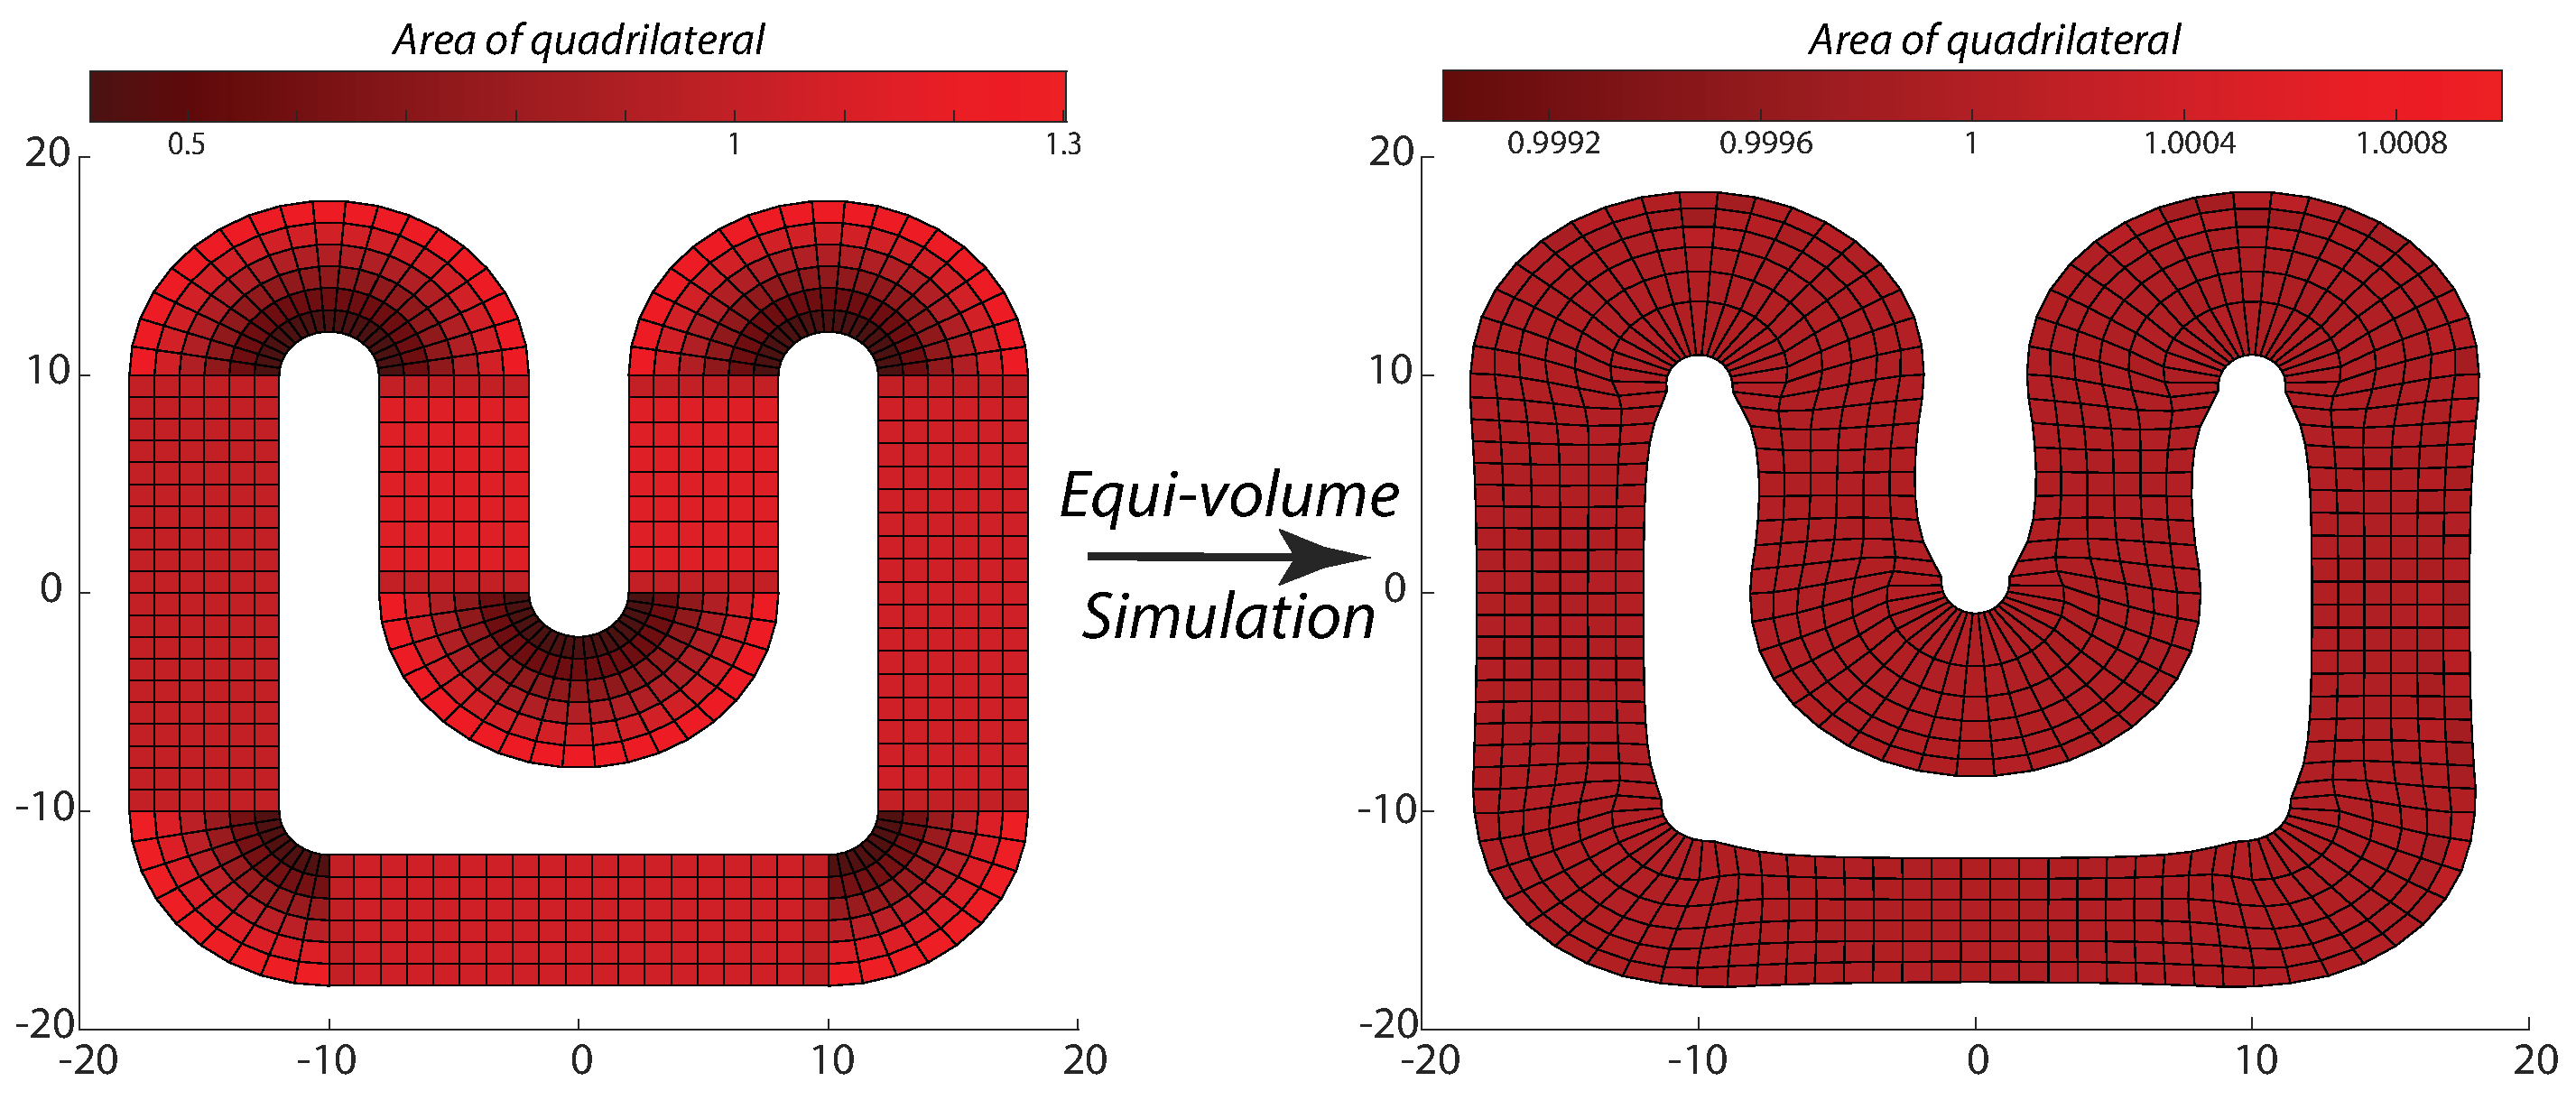
\includegraphics[width=1.\textwidth, clip=true]{./Chapters/03_GLM/./Images/Simulation}
\caption{From an initially equidistant mesh, on the left, we let the points on the mesh rearrange itself in an equivolume manner. The area of a single quadrilateral is indicated by its colour. The resulting mesh, on the right, is rearranged such that all quadrilaterals had unit area ($\pm 10^{-3}$). Note that as a result, the layers start varying in thickness in the inner and outer bends.}
\label{fig:simulation}
\end{figure}